

\begin{problem}

\textbf{\textsc{Relativistic Scattering}} A small spherical particle traveling at a speed $v=0.5c$ at an angle $\alpha=45^{\circ}$ from the horizontal is struck by an electromagnetic plane wave of angular frequency $\omega=7.08\times 10^{15} \;\mathrm{Hz}$ propagating directly to the right. In its own reference frame, the particle scatters light in all directions with the same frequency as the frequency of incident light it perceives. Due to the relativistic Doppler effect, however, the frequency of the scattered light measured in the lab frame is generally not the same as the incident light frequency. What is the angular frequency $\omega'$ of light scattered into a scattering angle of $\theta=89^{\circ}$? Assume the radius of the particle $R$ is small enough that $R\omega \ll c$.
\FloatBarrier
\begin{figure}[h]
    \centering
    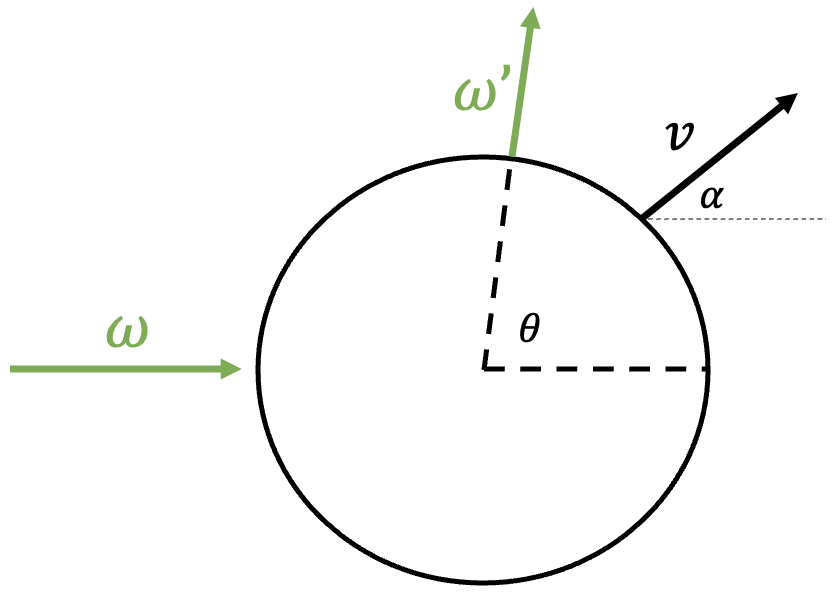
\includegraphics[width=0.4\linewidth]{problems/figures/rel_sca_fig.png}
    % \caption{Setup. Pictured is the scattering angle $\theta$ and the velocity $v$ of the particle. Contrary to what the coloring would suggest, the scattered light frequency $\omega'$ might not be the same as the incident light frequency $\omega$.}
    \label{fig:enter-label}
\end{figure}
\FloatBarrier
\end{problem}
